\documentclass[a4paper,14pt]{extarticle}
\usepackage[english,russian]{babel}
\usepackage[cache=false]{minted}
\usepackage{fontspec}
\usepackage{indentfirst}
\usepackage{listings}
\usepackage{color}
\usepackage{caption}
\usepackage{amsmath}
\usepackage{hyperref}
\usepackage{graphicx}
\usepackage[%
    left=20mm,%
    right=10mm,%
    top=20mm,%
    bottom=20mm,%
]{geometry}%
\usepackage{titlesec}


\setmainfont{PT Astra Serif}

\hypersetup{
    colorlinks=true,
    linkcolor=black,
    filecolor=magenta,
    urlcolor=cyan,
    pdftitle={Лабораторная работа №4},
    pdfpagemode=FullScreen,
}

\newcommand{\hlink}[2]{\href{#1}{\color{blue}\underline{#2}}}
\graphicspath{ {./images/} }

\setmonofont[Scale=0.8]{JetBrains Mono}
\setminted{frame=lines, framesep=3mm, fontsize=\small}
\usemintedstyle{vs}

\titleformat{\section}
{\normalfont\bfseries}{}{0pt}{Упражнение \thesection.\;}

\numberwithin{figure}{section}

\begin{document}

\begin{titlepage}
    \vspace{0pt plus2fill}
    \noindent

    \vspace{0pt plus6fill}
    \begin{center}
        \textbf{\large{Санкт-Петербургский национальный исследовательский университет информационных
                технологий, механики и оптики}}

        \vspace{0pt plus2fill}
        \textbf{\Large{ЛАБОРАТОРНАЯ РАБОТА №1}}

        \vspace{0pt plus2fill}
        \textbf{\large{Создание программы с помощью \\ среды разработки Visual Studio .NET}}
    \end{center}

    \vspace{0pt plus8fill}
    \begin{flushright}
        Студент: \\
        \textit{Швалов Даниил Андреевич}

        \textit{Факультет ИКТ}

        Группа: \textit{К32211}

        Преподаватель: \\
        \textit{Иванов Сергей Евгеньевич}
    \end{flushright}

    \vspace{0pt plus4fill}
    \begin{center}
        {Санкт-Петербург~--- 2023}
    \end{center}
\end{titlepage}

\section{Создание простой программы в текстовом редакторе}

Выполнив все шаги из задания, я получил следующий исходный код:
\inputminted{csharp}{../TextEditor/MyProgram.cs}

Для компиляции программы я использовал следующую команду:
\begin{minted}{shell}
    csc /out:MyHelloProgram.exe MyProgram.cs
\end{minted}

Здесь аргумент командой строки \texttt{/out:MyHelloProgram.exe} устанавливает имя выходного файла (по умолчанию это базовое имя файла с классом main или имя первого файла).

Запустив программу и введя имя, получим следующий вывод программы:
\begin{minted}{shell}
    Please enter your name
    Hello, Daniil
\end{minted}

\section{Создание программы с помощью среды разработки Visual Studio .NET}

Создав новое консольное приложение C\# в Visual Studio .NET, а также выполнив шаги из задания, я получил следующий исходный код:
\inputminted{csharp}{../Greetings/Greetings/Program.cs}

Запустив программу и введя имя, я получил вывод программы, представленный на рис. \ref{fig:task-2}.
\begin{figure}[H]
    \centering
    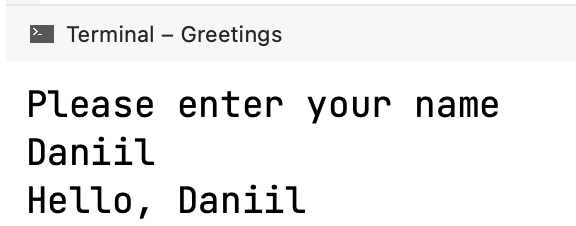
\includegraphics[width=0.7\textwidth]{images/task-2.png}
    \caption{Вывод программы Greetings}
    \label{fig:task-2}
\end{figure}

\section{Использование отладчика Visual Studio .NET}

На рис. \ref{fig:task-3-1} я добавил точку останова в месте, где впервые встречается команда \texttt{Console.WriteLine}.

\begin{figure}[H]
    \centering
    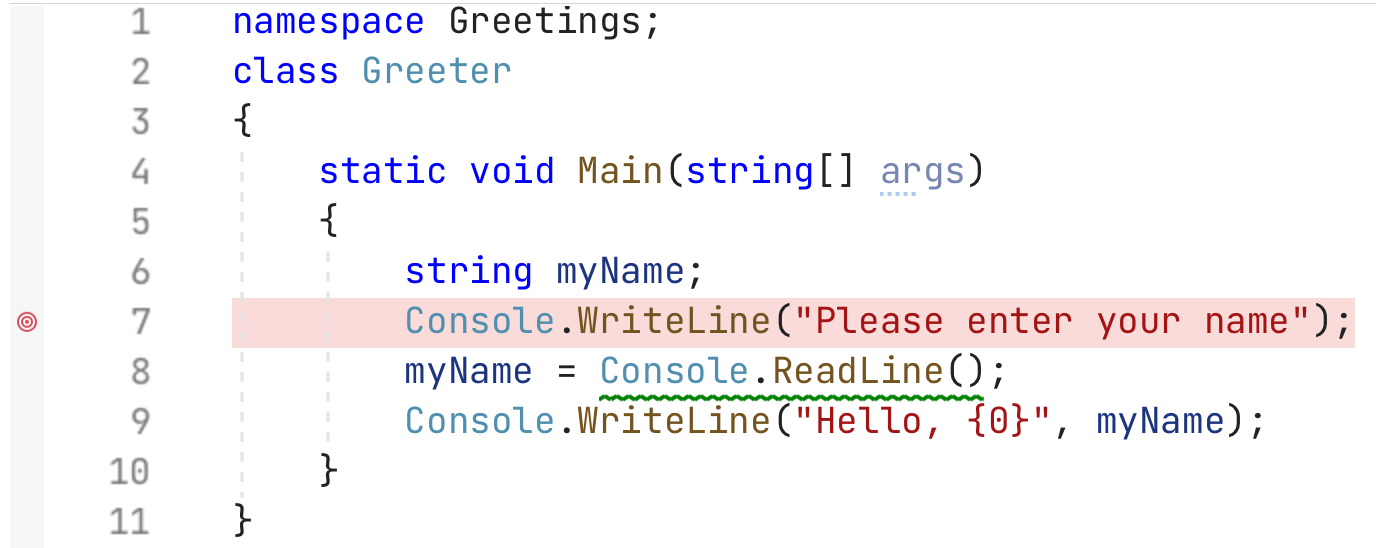
\includegraphics[width=\textwidth]{images/task-3-1.png}
    \caption{Добавление точки останова}
    \label{fig:task-3-1}
\end{figure}

На рис. \ref{fig:task-3-2} я добавил переменную \texttt{myName} в список выражений для мониторинга.

\begin{figure}[H]
    \centering
    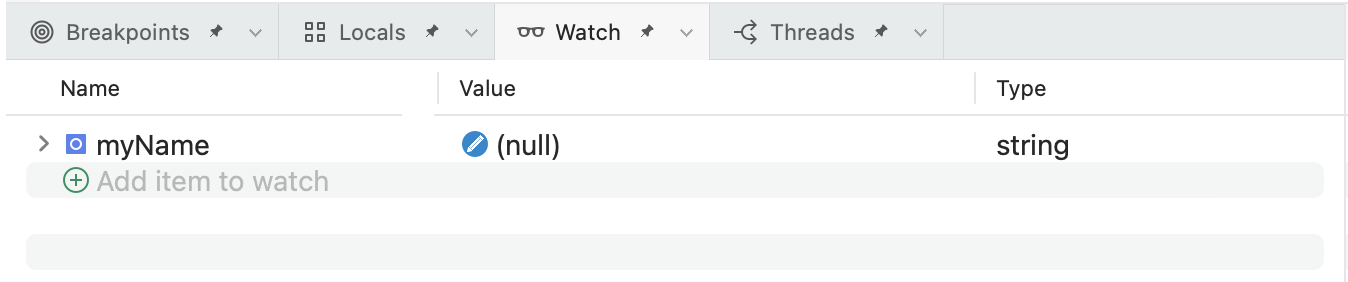
\includegraphics[width=0.9\textwidth]{images/task-3-2.png}
    \caption{Добавление переменной в мониторинг}
    \label{fig:task-3-2}
\end{figure}

На рис. \ref{fig:task-3-3} и рис. \ref{fig:task-3-4} я ввел имя, проверил значение переменной \texttt{myName} в отладчике.

\begin{figure}[H]
    \centering
    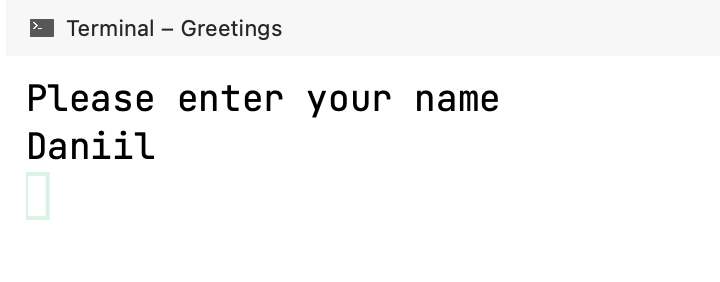
\includegraphics[width=0.7\textwidth]{images/task-3-3.png}
    \caption{Ввод имени}
    \label{fig:task-3-3}
\end{figure}

\begin{figure}[H]
    \centering
    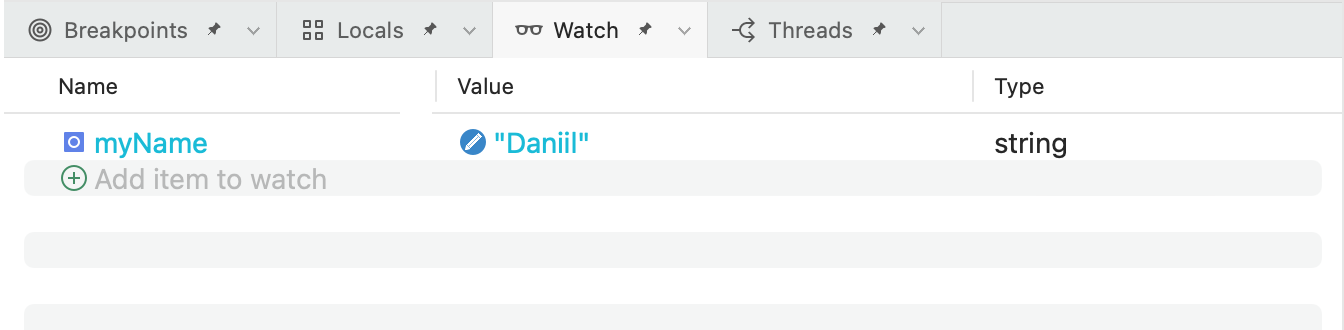
\includegraphics[width=0.9\textwidth]{images/task-3-4.png}
    \caption{Мониторинг значения переменной в отладчике}
    \label{fig:task-3-4}
\end{figure}

На рис. \ref{fig:task-3-5} я проверил вывод программы в консольном окне.

\begin{figure}[H]
    \centering
    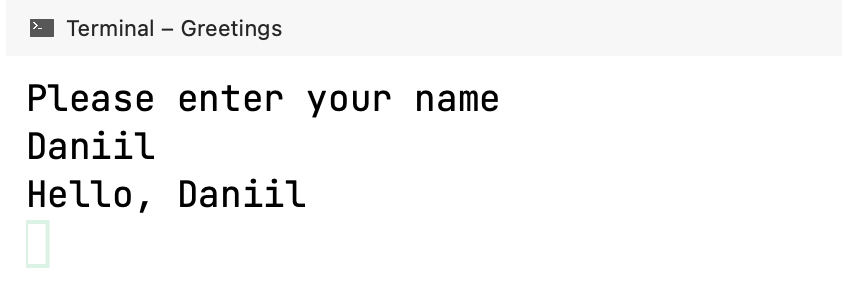
\includegraphics[width=0.7\textwidth]{images/task-3-5.png}
    \caption{Результат работы программы}
    \label{fig:task-3-5}
\end{figure}

\section{Добавление в C\#-программу обработчика исключительных ситуаций}

Проделав первые шаги, я получил следующую программу:
\inputminted{csharp}{../Divider/Divider/Program1.cs}

Я протестировал программу, введя числа \(10\) и \(5\), и получил корректный результат (см. рис. \ref{fig:task-4-1}).

\begin{figure}[H]
    \centering
    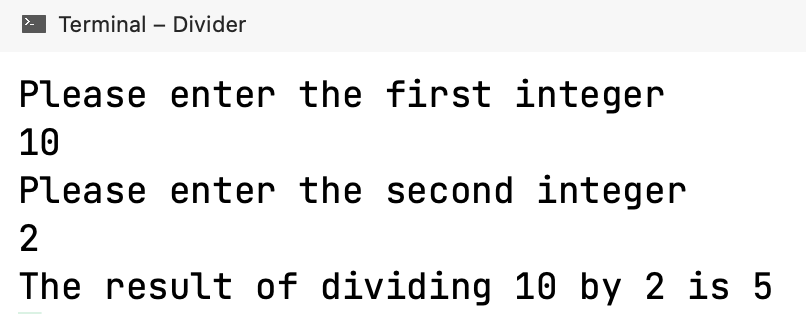
\includegraphics[width=0.7\textwidth]{images/task-4-1.png}
    \caption{Ввод чисел \(10\) и \(5\)}
    \label{fig:task-4-1}
\end{figure}

Затем я вновь протестировал программу, введя числа \(10\) и \(3\) (см. рис. \ref{fig:task-4-2}). Я получил не совсем корректный результат. Вместо \(3.33\) программа вывела \(3\). Это произошло потому, что для хранения чисел мы использовали целочисленный тип \texttt{int}. Поэтому при делении целых чисел мы также получили целое число вместо числа с плавающей запятой.

\begin{figure}[H]
    \centering
    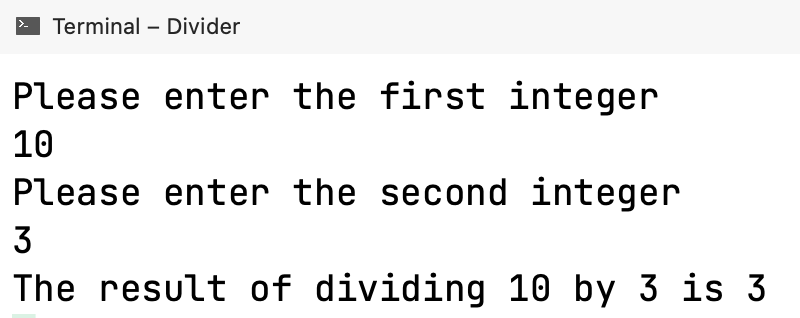
\includegraphics[width=0.7\textwidth]{images/task-4-2.png}
    \caption{Ввод чисел \(10\) и \(3\)}
    \label{fig:task-4-2}
\end{figure}

Теперь проверим что будет, если \(10\) разделить \(0\) (см. рис. \ref{fig:task-4-3}). В программе возникла исключительная ситуация.

\begin{figure}[H]
    \centering
    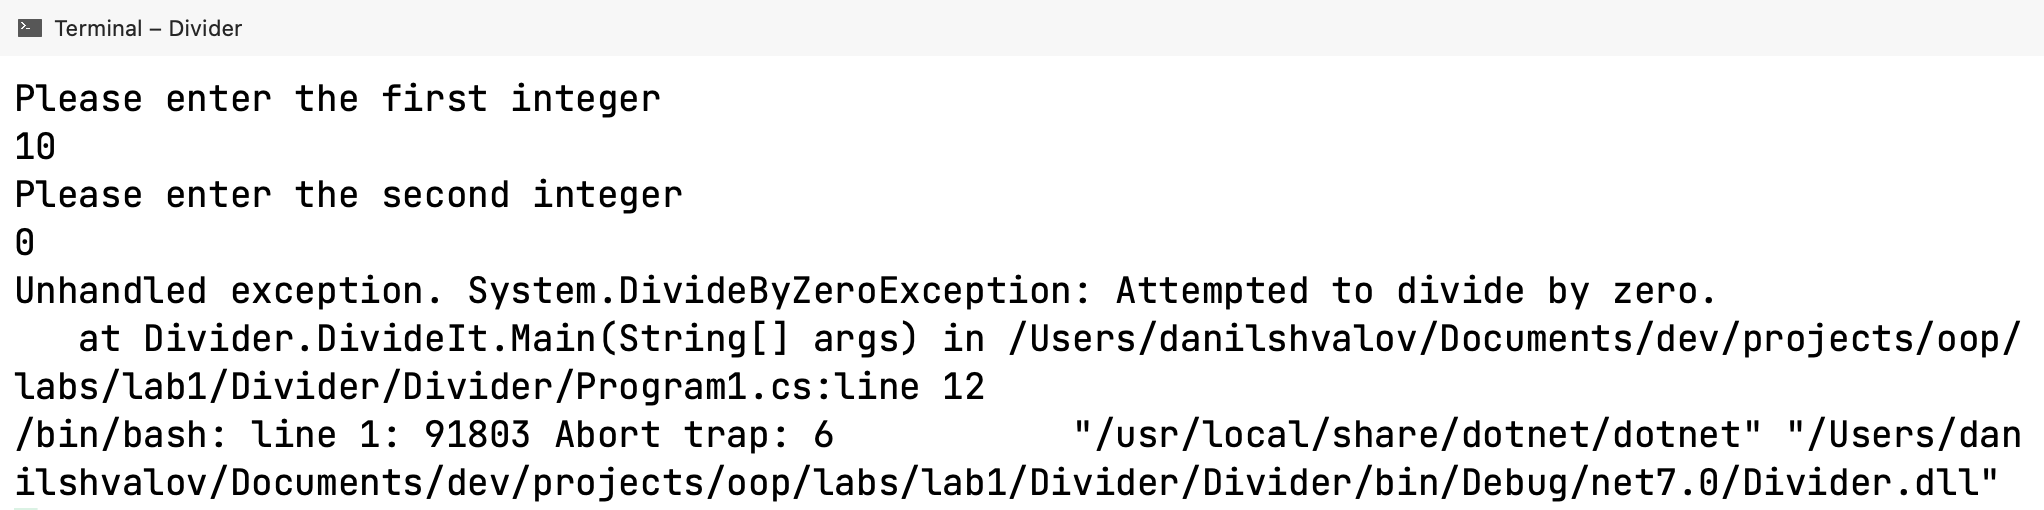
\includegraphics[width=0.7\textwidth]{images/task-4-3.png}
    \caption{Ввод чисел \(10\) и \(0\)}
    \label{fig:task-4-3}
\end{figure}

Добавим в программу обработчик исключительных ситуаций:
\inputminted{csharp}{../Divider/Divider/Program2.cs}

Теперь проверим работу программы при вводе \(10\) и \(0\) (см. рис. \ref{fig:task-4-4}). Программа обработала ошибку корректно.

\begin{figure}[H]
    \centering
    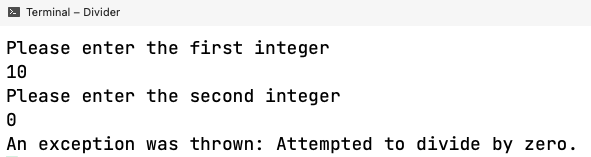
\includegraphics[width=0.7\textwidth]{images/task-4-4.png}
    \caption{Ввод чисел \(10\) и \(0\) после добавления обработчика}
    \label{fig:task-4-4}
\end{figure}

Теперь попробуем ввести букву вместо числа (см. рис. \ref{fig:task-4-5}). Программа также корректно обработала эту ситуацию.

\begin{figure}[H]
    \centering
    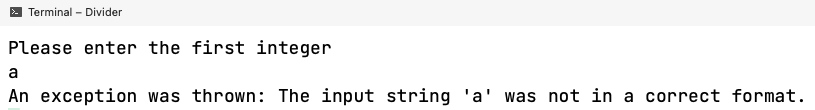
\includegraphics[width=0.7\textwidth]{images/task-4-5.png}
    \caption{Ввод буквы вместо числа}
    \label{fig:task-4-5}
\end{figure}

Добавим в программу обработчик исключительной ситуации при вводе данных неверного формата:
\inputminted{csharp}{../Divider/Divider/Program.cs}

Проверим программу и введем букву вместо числа (см. рис. \ref{fig:task-4-6}). Программа верно обработала эту ситуацию.

\begin{figure}[H]
    \centering
    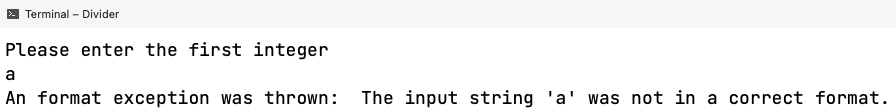
\includegraphics[width=0.7\textwidth]{images/task-4-6.png}
    \caption{Ввод буквы вместо числа}
    \label{fig:task-4-6}
\end{figure}

\section{Расчет площади треугольника}

В своей программе я считываю сторону треугольника в переменную \texttt{side}. После этого я создаю переменную \texttt{p} и присваиваю ей значение полу периметра треугольника. Для расчета площади треугольника я использую формулу Герона:
\[
    S = \sqrt{p (p - a) (p - b) (p - c)} = \sqrt{p (p - x)^3}.
\]
Нахожу площадь, сохраняю ее в переменную \texttt{square} и вывожу информацию в виде таблицы. Кроме того, в программе я обрабатываю исключительные ситуации и вывожу информацию об ошибках пользователю на экран. Пример использования программы представлен на рис. \ref{fig:task-5}.

\begin{figure}[H]
    \centering
    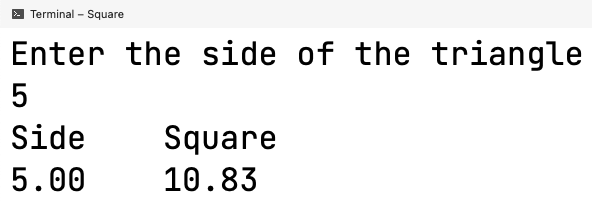
\includegraphics[width=0.7\textwidth]{images/task-5.png}
    \caption{Пример расчета площади}
    \label{fig:task-5}
\end{figure}

Исходный код программы представлен в следующем листинге:
\inputminted{csharp}{../Square/Program.cs}

\end{document}
